\chapter{Paraview}

ICE features functionality for visualizing models using ParaView.

\section{Installation and Configuration}

ParaView use for ICE requires a Mac OS or Linux operating system, as ICE does
not currently support ParaView connections on Windows. You will also need an
installation of ParaView on your local machine. ParaView can be downloaded from
its \href{http://www.paraview.org/download/}{official website}. The ICE
development team recommends using the latest available version of ParaView,
currently 5.0.1 at the time of this writing. You will further need a custom
Python HTTP web server implementation, which can be downloaded from the
\href{http://eclipseice.ornl.gov/downloads/paraview/scripts/http_pvw_server.py}{Oak
Ridge website}.

\subsection{Launching ParaView}  

Before connecting to ParaView, it must be launched from the command line. This
can be done by running the command:

\textbf{DISPLAY\=:0 (ParaView installation folder)/bin/pvpython (Path to web
server file)/http\_pvw\_server.py -{}-host localhost -{}-port 8600}.

On Mac, the first path should instead end in \newline
\textbf{/paraview.app/Contents/bin/pvpython} to specify the file inside of the
ParaView application.

This will launch the web server script in ParaView Python. You can specify a
different port as needed by using a different number after ``-port''.

\subsection{Configuring the ParaView Connection}

Once ParaView is running, ICE must be configured to connect to the server. This
is done through specifying a default connection in the ICE Preferences page.
This process only needs to be performed once. After initially creating the
connection, ICE will attempt to connect to ParaView on that port each time it is
launched.

To set the connection, select Window $\rightarrow$ Preferences\ldots in ICE's
menu bar. (On Mac OS X, Preferences\ldots is located under ICE instead of
Windows.) Select Visualization $\rightarrow$ ParaView in the tree on the left
side of the Preferences window.

\begin{center}
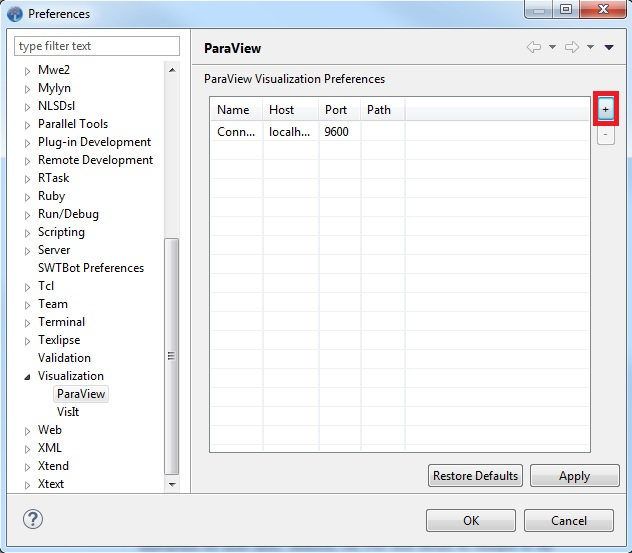
\includegraphics[width=12cm]{images/paraviewpreferencepage_ice}
\end{center}

Press the button with a ''+" symbol in the upper right (highlighted in the image
above) to add a new row to the table. Click on cells in the new row to edit
their values. The default values automatically supplied by ICE should be
appropriate for most users. However, the Port field should be changed to the
port number you specified when starting the server. (8600 if using the example
above.)

Once finished editing the cells in the new row, press Apply, then OK. ICE will
then connect to the ParaView server.

\section{Opening a ParaView File} 

To open a ParaView Plot Editor, a file that uses this editor must first be
placed in the Project Explorer. This view lists files imported into ICE. To
access the Project Explorer, use the the menu bar at the top of the window and
navigate to Window $\rightarrow$ Show View $\rightarrow$ Project Explorer.
Depending on the active Eclipse perspective, opening this view may require
selecting Other\ldots and finding the Project Explorer in the dialog under the
General category in the tree.

By default, the Project Explorer should automatically import the
ICEFiles/default and ICEFiles/itemDB folders. If it does not, or if you want to
import a different folder into ICE, right click in the Project Explorer and
select Import\ldots from the context menu. Then, select General $\rightarrow$
File System from the tree, and press the Next button. Select directories and/or
files to import into the Project Explorer, and enter which folder they should
be imported into, as shown below.

\begin{center}
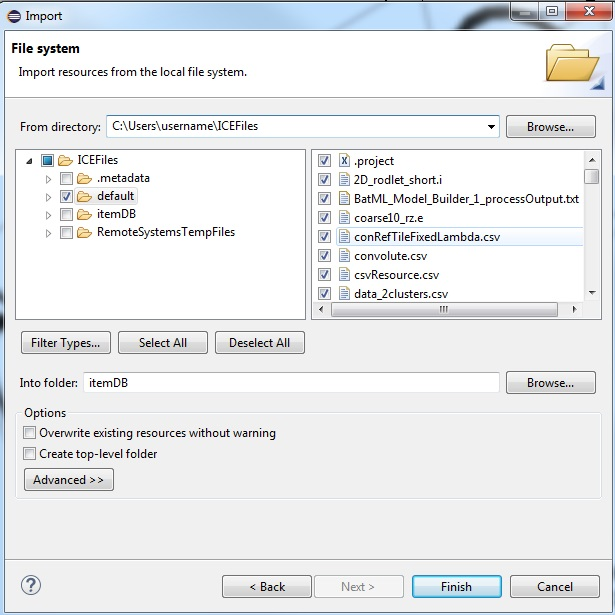
\includegraphics[width=12cm]{images/ImportFileDialog}
\end{center}

Once a file is in the Project Explorer, simply double click on it to open it in
ParaView.

\subsection{Using ParaView}

\subsubsection{Camera Controls}

The Plot Editor allows the user to rotate the model by clicking and dragging
inside the display area or adjust the zoom by scrolling the mouse wheel. Other
commands vary slightly between the two utilities.

\subsubsection{Selecting the Plot}

Pressing the Select Series\ldots button will open a dialog which lists the
various plots in the opened file. Simply select one and click OK to open it. 

\begin{center}
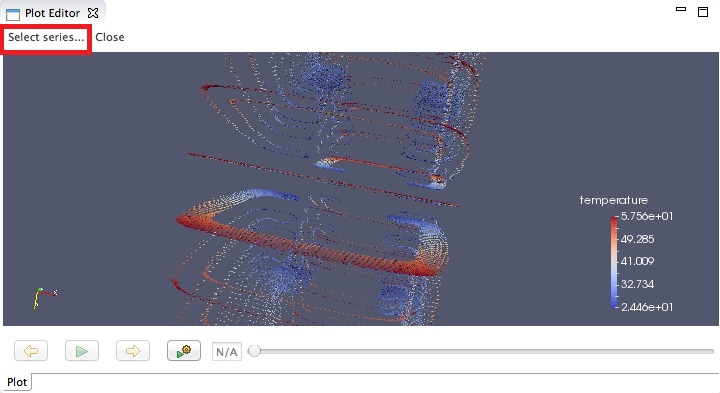
\includegraphics[width=12cm]{images/ParaViewPlotEditorSelectSeriesButton}
\end{center}

\subsubsection{Setting the Plot Representation} 

ParaView is capable of displaying plots in several different representations,
such as points or surfaces. To switch between plot type, right click inside the Plot
Editor's display area and select one of the listed options under the
Representation category in the context menu.

\begin{center}
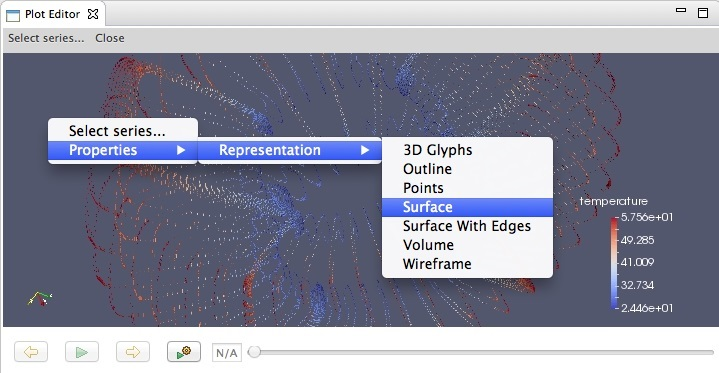
\includegraphics[width=12cm]{images/ParaViewRepresentationDropDown}
\end{center}

\subsubsection{Animation and Time Data}

The Plot Editor features a time slider widget at the bottom of the screen. 

\begin{center}
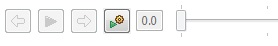
\includegraphics[width=12cm]{images/TimeSliderWidget}
\end{center}

The controls, in order of left to right, are:

1) Return to the previous time step.

2) Automatically play the plot as an animation by displaying the time steps
sequentially. 

3) Advance to the next time step. 

4) Opens an options menu that allows the user to set the playback speed, toggle
whether the animation should loop when it reaches the end, and set the plot to
the first or last time step.

5) A display for the current time step. It can be edited to set the plot to an
arbitrary time step. 

6) A slider that shows the current time step's position on the timeline. The
slider can be dragged around the timeline, setting the plot's time step
accordingly.

\section{Accessing a ParaView Web Server}

It is also possible to access the full ParaView web viewer application inside of
ICE. This allows for full access to all the web viewer's features and for remote
connections to another machine hosting the ParaView session, even for Windows
clients.

\subsection{Launching the ParaView Web Visualizer}

Before connecting, the visualizer needs to be started from the command line.
ParaView's package structure is different on each operating system,
neccesitating a different command for each.

For the following commands, replace paraview-install with the path to your
machine's ParaView installation and data-folder with the path to the top level
folder under which all files you wish to visualize are kept.

For \textbf{Linux} run:

\textbf{paraview-install/bin/pvpython
paraview-install/lib/paraview-5.0/\newline
site-packages/paraview/web/pv\_web/visualizer.py -{}-content
paraview-install/share/paraview-5.0/www/ -{}-data-dir data-folder/ -{}-port
8600}

For \textbf{Mac OS} run:
 
\textbf{paraview-install/paraview.app/Contents/bin/pvpython
paraview-install/paraview.app/Contents/Python/paraview/web/\newline
pv\_web\_visulizer.py -{}-content
paraview-install/paraview.app/\newline Contents/www/ -{}-data-dir data-folder/
-{}-port 8600}

In all cases, the arguement following ``--port'' can be changed to set the port
number the server will use.

\subsection{Accessing the Visualizer}

Now that the visualizer is running, it can be accessed by the client machine,
which may be the same machine running the server.

Within ICE, click Window $\rightarrow$ Show View $\rightarrow$ Other\ldots to
open a dialog of views. Select General $\rightarrow$ Internal Web Browser from
it and press OK.

Finally, navigate to http://hostname:8600/apps/Visualizer inside the browser,
replacing the hostname and port number as appropriate. 

\subsection{Using the Visualizer}

In order to load a data file, click the Show File List button as seen below.

\begin{center}
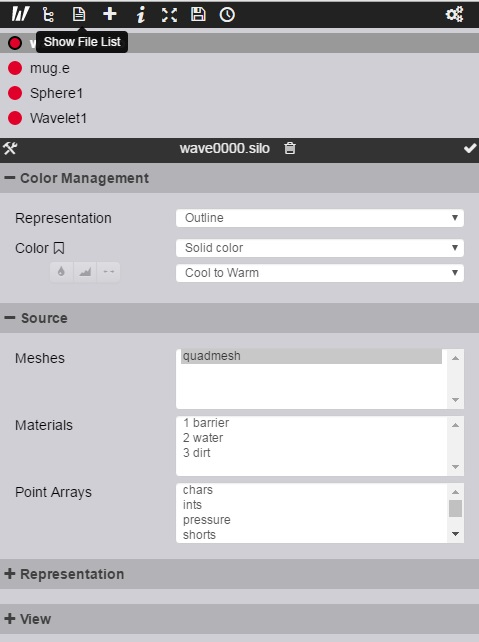
\includegraphics[width=12cm]{images/ParaViewVisualizer}
\end{center}

This will place the contents of the folder specified by the --data-dir arguement
when launching the visualizer into the side bar. You may then double click on a
file to load it into the model. 

You can click and drag the mouse to rotate the camera and right click followed
by dragging up or down to zoom. A full description of the visualizer's features
are beyond the scope of this tutorial, but see the official documentation
\href{http://www.paraview.org/ParaView3/Doc/Nightly/www/js-doc/index.html#!/guide/web_visualizer}{here}.